\documentclass[10pt,a4paper]{article}

\usepackage{afterpage}
\usepackage{pgfplots}
\usepackage{siunitx}
\usepackage{tikz}
\usepackage{amsmath}
\usepackage{amssymb}
\usepackage{nomencl}
\usepackage{url}
\usepackage{listings}
\usepackage{color}
\usepackage{caption}
\usepackage{subcaption}
\usepackage{float}
\usepackage[margin=1in]{geometry}
\usepackage{multirow}
\usepackage{graphicx}
\makenomenclature

\definecolor{dkgreen}{rgb}{0,0.6,0}
\definecolor{gray}{rgb}{0.5,0.5,0.5}
\definecolor{mauve}{rgb}{0.58,0,0.82}

\lstset{frame=tb,
	language=C++,
	aboveskip=3mm,
	belowskip=3mm,
	showstringspaces=false,
	columns=flexible,
	basicstyle={\small\ttfamily},
	numbers=none,
	numberstyle=\tiny\color{gray},
	keywordstyle=\color{blue},
	commentstyle=\color{dkgreen},
	stringstyle=\color{mauve},
	breaklines=true,
	breakatwhitespace=true,
	tabsize=3
}


\pgfplotsset{compat=newest} % Allows to place the legend below plot
\usepgfplotslibrary{units} % Allows to enter the units nicely

\sisetup{
	round-mode          = places,
	round-precision     = 2,
}

\numberwithin{equation}{section}

\makeindex

\pagenumbering{gobble}
\begin{document}
	
	\begin{titlepage}
		
		\newcommand{\HRule}{\rule{\linewidth}{0.5mm}} % Defines a new command for the horizontal lines, change thickness here
		
		\center % Center everything on the page
		
		\textsc{\LARGE Cranfield University}\\[1.5cm] % Name of your university/college
		\textsc{\Large Computational and Software Techniques in Engineering}\\[0.5cm] % Major heading such as course name
		\textsc{\large Gruop Project}\\[0.5cm] % Minor heading such as course title
		
		\HRule \\[0.4cm]
		{ \huge \bfseries Assignment}\\[0.4cm] % Title of your document
		\HRule \\[1.5cm]
		
		\begin{minipage}{0.4\textwidth}
			\begin{flushleft} \large
				\emph{Authors:}\\
				Benjamin \textsc{Deguerre}\\
				Wojciech \textsc{Jonczyk}\\ % Your name
				Alix \textsc{Kamano}\\
				Anna \textsc{Zaporowska}
			\end{flushleft}
		\end{minipage}
		~
		\begin{minipage}{0.4\textwidth}
			\begin{flushright} \large
				\emph{Supervisor:} \\
				Dr. Chi chun gilbert \textsc{Tang} % Supervisor's Name
			\end{flushright}
		\end{minipage}\\[2cm]
		
		{\large 10 December 2016}\\[3cm] % Date, change the \today to a set date if you want to be precise
		
		
\includegraphics{logo}\\[2cm] % Include a department/university logo - this will require the graphicx package
		
		
		\vfill % Fill the rest of the page with whitespace
		
	\end{titlepage}

\tableofcontents
\section{Introduction}
\begin{figure}[H]
	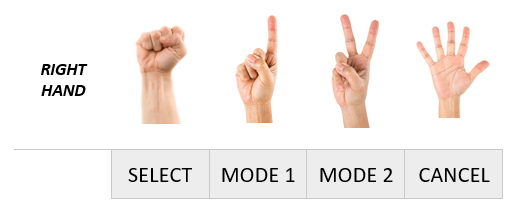
\includegraphics{mode_selection}
	\centering
	\caption{Mode selection - set of gestures}
	\label{fig:mode}
\end{figure}
\newpage
\section{Mode 1 - Static mode}
\subsection {Mode description}
The first mode allows user to select and write proper letter. In english alphabet there are 26 letters, so to be able to use all of them a lot of gestures had to be specified and implemented. Our aim was to do this as simple as possible, because too complicated set of movements and signs could have not been user-friendly and straightforward. The scheme was shown in the Figure \ref{fig:letters}.

\begin{figure}[H]
	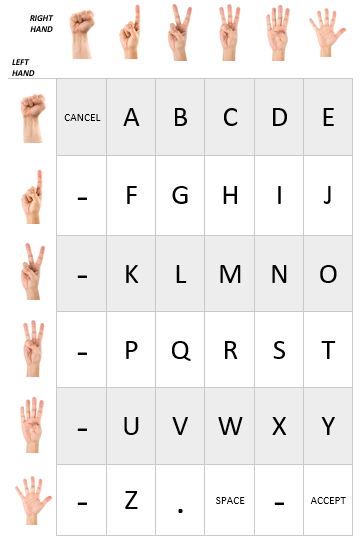
\includegraphics{static_gestures}
	\centering
	\caption{Letter selection - set of gestures}
	\label{fig:letters}
\end{figure}

Every letter and command had its own and unique command. \textbf{By counting number of extended fingers in either hands differentation was done}. It was very clear and easy to learn set of gestures. For instance, when in the left hand only one finger was extended and in the same moment the right hand was fully open then it meant that letter "J" should have been drawn. The system worked well only when leap was detecting both hands.\\

Sometimes wrong letter was selected and to avoid wrong comunication with the robot two additional gestures were added - command "Accept" to send proper letter to the robot and command "Cancel" to reset current letter and repeat selection. We wanted also to write full sentences. Thus we decided to implement gesture to draw dot and one more to make space between two words. It is easy to see in the Figure \ref{fig:letters} that there are 6 more possible gestures that were not used. That set of gestures can be easily extended. 

\subsection{Letters library}

\mbox{}\\

Additionally to mode architecture, letters library has been created. This library is in fact a set of movements which have to be done by the robot in order to write each of the letters. Each set of movements includes moving in all out of three dimensions (x, y, z). Letters library is built in such way that every letter is written in a rectangle of sides length of b and a, and left down corner coordinates of (c, d). After finishing movements for each letter, last move is always created to obtain new starting position for next letter, so the point (c, d) is updated with every new letter. It allows robot to write letters next to each other, which makes writing words or sentences possible. Starting point (c,d) as well as z1 and z2 (z dimension for robot being up, as a position when marker is not touching the surface, and down – in writing position) and sides lengths of a and b might be specified by user at the beginning of this program, which makes it more universal and multifunctional.\\

\begin{figure}[H]
	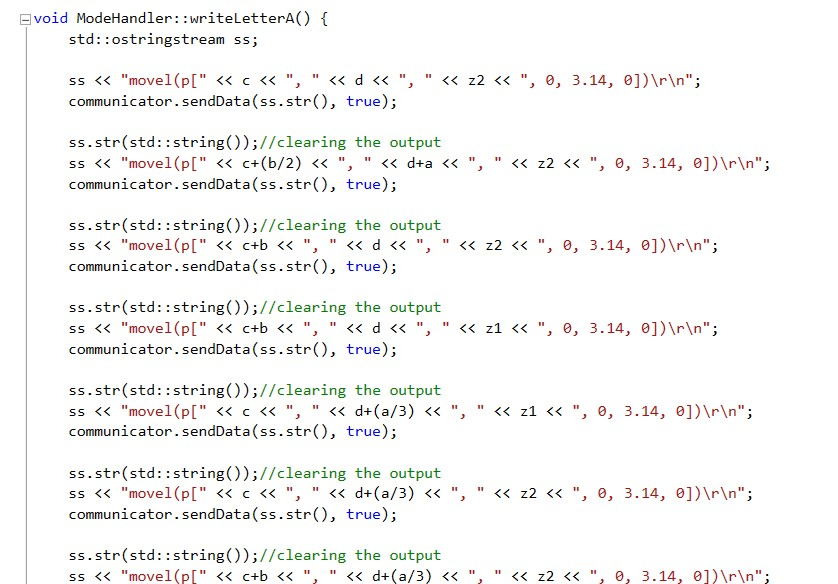
\includegraphics[scale=0.8]{Aletter}
	\centering
	\caption{Example code from letter library}
	\label{fig:Aletter}
\end{figure}

\mbox{}\\

Functions \textit{writeLetter} are constructed in such way that the whole commend is send to the robot controller, in this case it is the command \textit{movel(p[x, y, z, 0, 3.14, 0]}. This kind of communication was chosen because of easier access and possibilities of changing coordinates of starting point (c, d), which is crucial part for project main idea and was not possible or much more complicated to finish using other methods of working with robot. What is more, function \textit{movel} was chosen because of its functionality – this function makes robot move in straight line, without changing position of robot’s head (which is the main difference between other command \textit{movej} which reaches the target position in the shortest possible way, which is not necessarily the straight line). After sending the command delay between sending next command is given in order to allow robot to finish the first task, then the output is cleared, thus next command may be send. Without delay, robot’s controller after receiving pack of commands would perform only the last one, which means that the idea of using delay is crucial for program operation.  Example function for writing letter is given in the Figure \ref{fig:Aletter}. \\

Result of this set of movement is given in Figure \ref{fig:letter}. which shows the letter A written by robot’s arm after Leap Motion recognised gesture responsible for enable mode 1, then gesture responsible for letter A and gesture of acceptance. Inaccuracies visible in the Figure  \ref{fig:letter}. result from inappropriate marker placement, and not because of the program and could be improved in case of other program tests. \\

\begin{figure}[H]
	\includegraphics{Letter}
	\centering
	\caption{Example code from letter library}
	\label{fig:letter}
\end{figure}

\mbox{}\\

Prepared letters library is only one example of possible library which could be created for this kind of program. Since designed gestures are meant to be simple and intuitive for any user they can be used with other libraries like handwritten letters, small letters, numbers and any non-Latin alphabet etc., which makes this program more universal and user-friendly. Set of gestures are not too difficult to obtain, but need time to be prepared correctly. Its main advantage is the fact that one they are written, there is no need to worry about robot’s movements after launching the program. To make it easier for user, in case of future work, additional application could be proposed, which would automatically prepare set of gestures and save them in program’s memory. 

\newpage
\section{Mode 2 - Hand tracking}
adasdasdadad
\newpage	
\chapter{Conclusion}

\newpage

\end{document}
